Πριν να εξηγήσουμε τον τρόπο κατασκευής και λειτουργίας του PiLock, είναι αναγκαίο να αναφερθούμε στον τρόπο λειτουργίας των περισσότερων κλειδαριών σπιτιών, πολυκατοικιών ή και γραφείων.

Το σύστημα ξεκλειδώματος που χρησιμοποιείται στις περισσότερες κατοικίες αποτελείται από 2 εντελός ξεχωριστά και ανεξάρτητα συστήματα: Το σύστημα του θυροτηλεφώνου, δηλαδή το σύστημα μέσω του οποίου γίνεται η αναγνώριση του επισκέπτη (μέσω φωνής ή/και εικόνας), και το σύστημα ενεργοποίησης της κλειδαριάς. Στην παρούσα διατριβή θα αναφερθούμε αποκλειστικά στο δεύτερο σύστημα.

Οι ηλεκτρικές κλειδαριές που χρησιμοποιούνται σε πολυκατοικίες συνήθως αποτελούνται από ένα μάνταλο το οποίο, όταν το σύστημα ενεργοποιηθεί μέσω ρεύματος, απελευθερώνεται με αποτέλεσμα να μπορεί ελεύθερα η πόρτα να ανοίξει.

\begin{figure}[h]
	\centering
		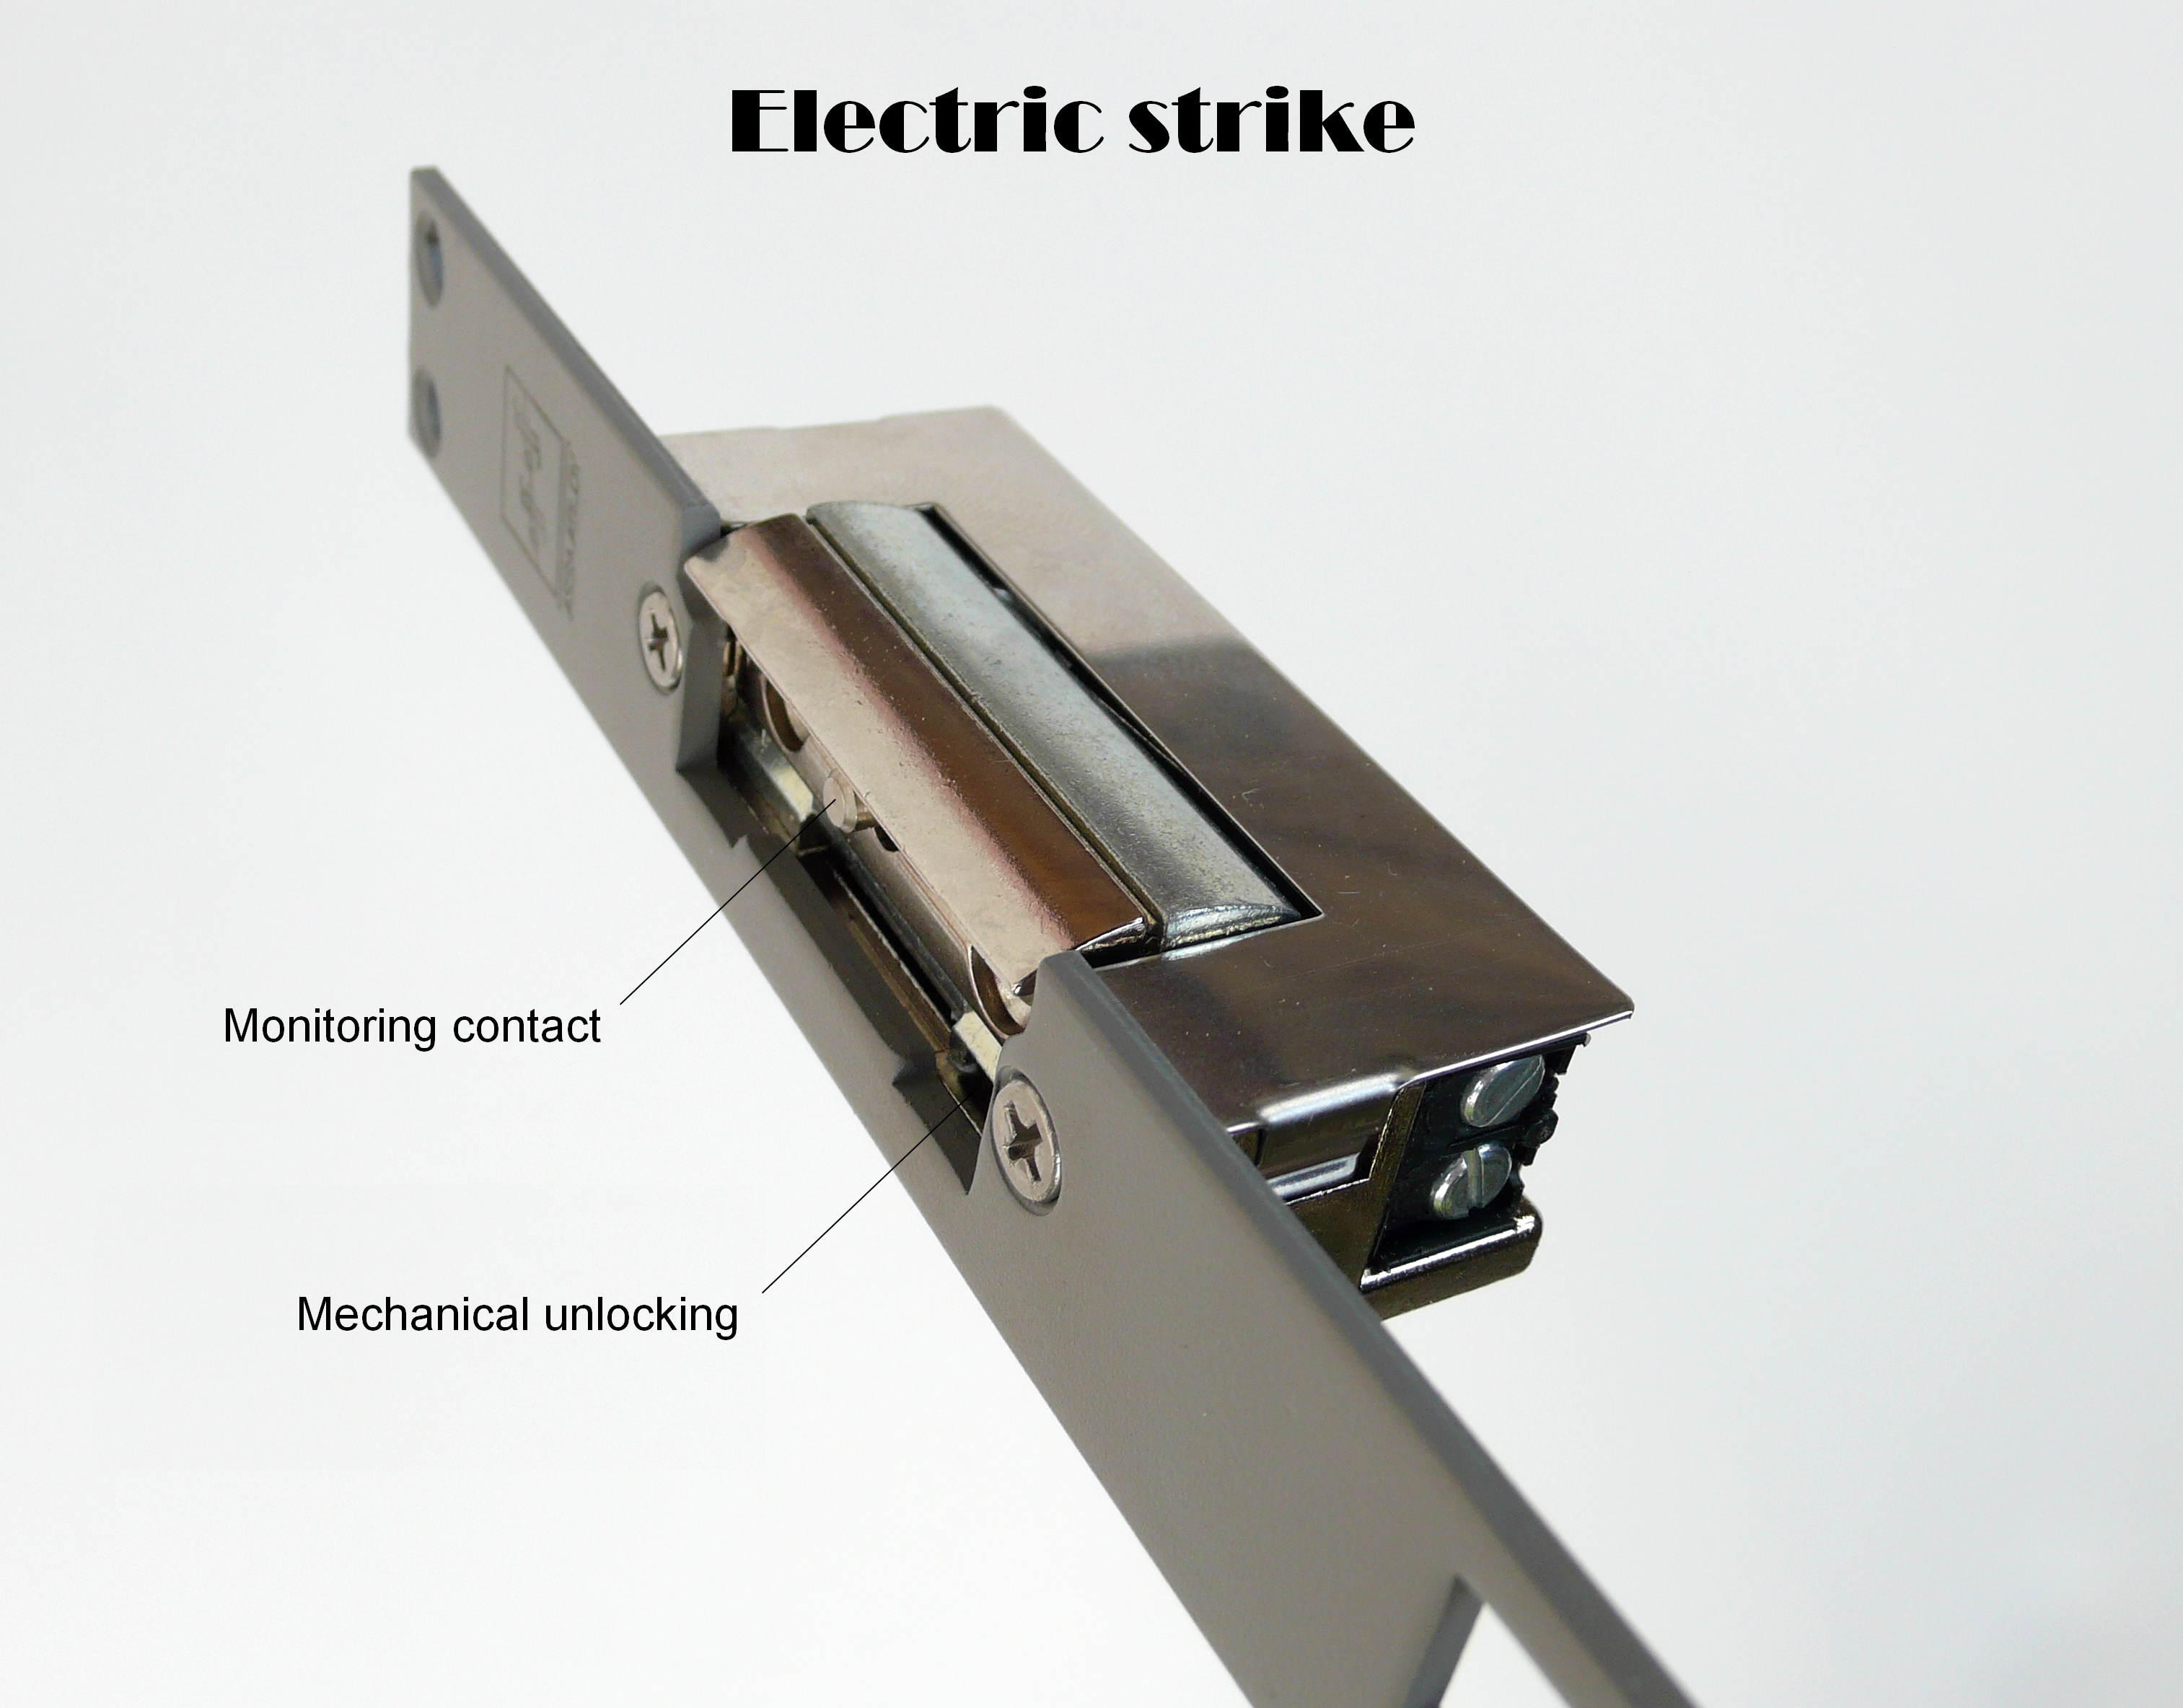
\includegraphics[width=0.5\textwidth,height=0.5\textheight,keepaspectratio]{Electric_strike.jpg}
	\caption{Ηλεκτρική κλειδαριά πολυκατοικίας με σύστημα καταγραφής κατάστασης κλειδώματος}
\end{figure}

Η ενεργοποίηση του παραπάνω συστήματος γίνεται μέσω ενός διακόπτη αναρτημένου πάνω στο θυροτηλέφωνο του κάθε διαμερίσματος. Η τροφοδοσία των συστημάτων αυτών μπορεί να γίνεται είτε μέσω απευθείας τροφοδοσίας από το ηλεκτρικό δίκτυο, είτε μέσω κάποιου μετασχηματιστή σε χαμηλότερες τάσεις.

Πλέον είναι προφανές πως μπορούμε να περάσουμε έναν 2ο διακόπτη παράλληλα με τον ήδη υπάρχον και να διαχειριστούμε εύκολα το σύστημα ξεκλειδώματος.